% Section 02 - Schrodinger problem for dressed quantum Hall system

Our system consists of a 2DEG placed on the $xy$-plane of the three-dimensional coordinate space. In our analysis, the 2DEG is subjected to a nonoscillating magnetic field $\vb{B} = (0,0,B)^{\text{T}}$ which is pointed towards the $z$ axis. In addition, a linearly polarized strong light is applied perpendicular to the 2DEG surface. We specially select the frequency of the dressing field $\omega$ to be in the off-ersonant regime such that the field behaves as a purely dressing field. Furthermore, without limiting the generality we choose $y$-polorized electric field $\vb{E} = (0,E\sin(\omega t),0)^{\text{T}}$ for the linearly polarized dressing field (Fig.~\ref{fig_1}).
\begin{figure}[b]
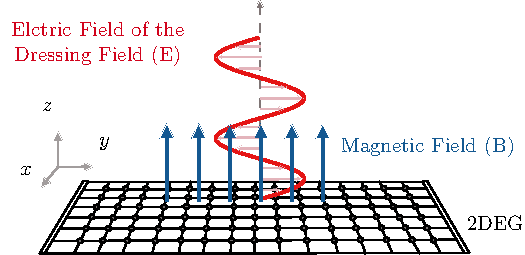
\includegraphics[scale=0.9]{figures/fig_1}
\caption{\label{fig_1} Our 2DEG system only confined in the $(x,y)$ plane while both stationary magnetic field $\vb{B}$ and dressing field (with y-polarized electric field $\vb{E}$) are applied perpendicular to the surface of 2DEG.}
\end{figure}
Here $B$ and $E$ represent the amplitudes of the stationary magnetic field and oscillating electric field respectively.

Using Landau gauge for the stationary magnetic field, we can represent it as a vector potential $\vb{A}_{s} = (-By,0,0)^{\text{T}}$. Furthermore, we model the dynamic dressing field in the Coulomb gauge as $\vb{A}_{d}(t) = (0,[E/\omega ]\cos(\omega t),0)^{\text{T}}$. These vector potentials are coupled to the momentum of 2DEG as kinetic momentum \cite{mahan00,bruus04}. Thus, our system can be represented with a time-dependent Hamiltonian
\begin{equation} \label{eq_1}
  \hat{H}_e(t) = \frac{1}{2m_e}\Big[\hat{\vb{p}} - e\big[\vb{A}_{s}+\vb{A}_{d}(t)\big]\Big]^2,
\end{equation}
where $m_e$ is the effective electron mass, $e$ is the magnitude of the electron charge, and $\hat{\vb{p}} = (\hat{p}_x,\hat{p}_y,0)^{\text{T}}$ represents the canonical momentum operator for 2DEG with electron momentum $(p_{x},p_{y},0)^{\text{T}}$.
The exact solutions for the time-dependent Schrödinger equation $i\hbar\; \text{d}\psi/\text{d}t = \hat{H}_e(t) \psi$ were already derived in Refs. \cite{husimi53,ditt98,dini16}. Here we present them as a set of wave functions defined by two quantum numbers $(n,m)$
\begin{equation} \label{eq_2}
  \begin{aligned}
    \psi_{n,m}&(x,y,t)  \\
    & = \frac{1}{\sqrt{L_x}}
    \chi_n\big(y - y_0 - \zeta(t)\big)\\
    & \times
    \text{exp}\bigg(
    \frac{i}{\hbar}\bigg[- \epsilon_n t
    + p_x x + \frac{eE[y - y_0]}{\omega}\cos(\omega t)\\
    &+
    m_e\dot{\zeta}(t)\big[y - y_0 -\zeta(t)\big] +
    \int_0^{t}dt'L(\zeta,\dot{\zeta},t')\bigg]\bigg),
  \end{aligned}
\end{equation}
where $n \in \mathbb{Z}^{+}_0$ and $m \in \mathbb{Z}$. Here $L_{x}$ and $L_{y}$ are dimensions of the 2DEG surface, and $\hbar$ is the reduced Planck constant. The center of the cyclotron orbit on the $y$-axis is given by $y_0 = -p_x/eB$ with $p_x = 2\pi \hbar m/L_x$.
Moreover, $\chi_n$ are well known eigenstate solutions for the Schrödinger equation of the stationary quantum harmonic oscillator
\begin{equation} \label{eq_3}
  \chi_n(y) =
   \frac{\sqrt{\kappa}}{\sqrt{2^{n}n!}}
  e^{-\kappa^2 y^2/2}
  \mathcal{H}_n \qty(\kappa y) \quad \text{with}
  \quad
  \kappa = \sqrt{\frac{m_e \omega_0}{\hbar}},
\end{equation}
with eigenvalues $\epsilon_n = \hbar \omega_0 (n + 1/2)$ where $\omega_0 = eB/m_e$ being the cyclotron frequency and $\mathcal{H}_n(\cdot)$ is the $n$-th Hermite polynomial.
The path shift of the driven classical oscillator $\zeta(t)$ is given by
\begin{equation} \label{eq_4}
  \zeta(t) = \frac{eE}{m_e(\omega_0^2 - \omega^2)}\sin(\omega t),
\end{equation}
while the Lagrangian of the driven classical oscillator $L(\zeta,\dot{\zeta},t)$ can be identified as
\begin{equation} \label{eq_5}
  L(\zeta,\dot{\zeta},t) = \frac{1}{2} m_e\dot{\zeta}^2(t) - \frac{1}{2}m_e\omega_0^2 \zeta^2(t) + eE\zeta(t) \sin(\omega t).
\end{equation}
For details of the full derivation refer to Appendix \ref{appendix_a}.
The exponential phase shifts in Eq.~(\ref{eq_2}) represent the influence of the stationary magnetic field and dressing field on the electron behavior of our system. Therefore, we can observe that the magneto-transport characteristics of 2DEG can be renormalized by a nonoscillating magnetic field along with a dressing field.
